\chapter{Implementace} 
\label{chap:implementation}
V této části je popsána implementace celého systému. Vzhledem k faktu, že většina rozhodnutí byla již učiněna ve fázi návrhu, tak zde budou pouze nastíněny problémy, které se při implementaci vyskytly, a jak byly řešeny. 

\section{Stahování a aktualizace dat}
Vzhledem k tomu, že se jedná o~data centrickou aplikaci, tak je tento subsystém v rámci celé aplikace velmi kritický. Většinu scrapovacích pavouků se povedlo rozšířit o~získávání URL adres snímků, ale u~některých to vedlo na více HTTP dotazů pro získání jednoho záznamu. V~rámci některých archivů je nutné provést dodatečný dotaz předtím, než je možné zobrazit snímek, proto v~doménovém modelu entita snímku obsahuje položku \texttt{preFetchUrl}. Jedním z~velmi omezujících požadavků na systém bylo, že má uchovávat pouze odkazy na původní datové úložiště, jelikož data sesbíraná z~více archivů by kladla velké požadavky na kapacitu úložiště. Ve výsledku se jednalo o největší problém v~rámci řešení daného systému, jelikož jednotlivé archivy používají různé formáty a~typy uložení, což vyžadovalo mnoho práce na straně jak samotných scraperů, tak i~na straně klientské aplikace, která se musela postarat o~bezproblémové zobrazení různorodých formátů.

\subsection{Lokality}
Každý archivní materiál je navázán na jednotlivé obce, ale většina archivních systémů poskytuje informaci pouze o~názvu obce. Samotný název obce bohužel nestačí k~přesné identifikaci obce, jelikož názvy obcí nejsou unikátní. Prvotní myšlenka, jež byla nastíněna vedoucím práce, spočívala ve využití jedinečných identifikátorů RÚIAN. Tento přístup narážel na problém, že daný systém identifikátorů se používá pouze na území České republiky a mnoho archiválií, které se nacházejí v~pohraničních archivech, obsahuje města i~v~zahraničí. Další problém tohoto přístupu spočíval v~tom, že identifikátor RÚIAN je sice unikátní, ale tím, že ho archivní weby neuvádějí, tak je nezbytné RÚIAN vyhledat podle nascrapovaných dat. V~případě získání více shod na název obce, není možné jednoznačně určit jaký záznam zvolit. Odpověď nelze ohodnotit podle korektnosti shody a následně porovnat jednotlivé shody. Vhodným ukazatelem by mohl být kraj nebo okres, kde se daná obec nachází. Problém je, že kraje a okresy se v průběhu času formovaly a posouvaly se jednotlivé hranice, takže není zaručeno, že Moravský zemský archiv obsahuje záznamy pouze z~Jihomoravského kraje. Na základě tohoto zjištění bylo nutné od identifikace pomocí RÚIAN ustoupit a~hledat alternativní přístup. Jako alternativní přístup bylo zvoleno použití zeměpisných souřadnic jednotlivých obcí a~porovnání vzdálenosti od archivu, který danou archiválii uchovává.
\newpara
V první řadě tedy bylo potřeba z informací dostupných pomocí scrapování získat jednotlivé obce. Proces přeměny adresy na zeměpisné souřadnice se nazývá geokódování a~existuje několik poskytovatelů, kteří tuto službu nabízí. V rámci České republiky se jedná například o \href{https://www.mapy.cz}{Mapy.cz}, které poskytují pravděpodobně nejdetailnější informace o oblastech na našem území, a to včetně již zaniklých obcí. Použití geolokačního API od \href{https://www.mapy.cz}{Mapy.cz} by se jevilo jako nejlepší možná volba, kdyby se od určitého vytížení za službu nemuselo platit. Za tímto účelem bylo využito geolokační API od neziskové organizace \href{https://www.openstreetmap.org/}{OpenStreetMap.org}, které je plně zdarma. Mezi hlavní problémy tohoto poskytovatele patří fakt, že jej plní lidé, tudíž se zde vyskytují často chybné či neúplné informace. Další limitace tohoto poskytovatele je, že v~rámci podmínek vkládání nových záznamů zakazuje vkládat historické názvy a jeho snahou je mapovat pouze aktuální lokality, což vzhledem k našemu řešenému problému představuje velkou komplikaci. Geokódovací API funguje podobně jako vyhledávač, takže v případě, že je vložena adresa, je získáno více možných výsledků. Vzhledem k tomu, že se jedná o~volání další externí služby, jež vytváří velkou prodlevu, tak jsou výsledky memorizovány a~v~případě, kdy je zavolán dotaz na shodnou adresu, tak se použije hodnota, kterou vrátila služba naposledy. Pro zvýšení přesnosti se v~rámci dotazu posílá poloha archivu jako středový bod, poblíž kterého se mají výsledky hledat.
\newpara 
Dalším krokem je tedy algoritmicky rozhodnout, jaký výsledek je správný, a to se snahou o~minimalizaci chybovosti. Navržený algoritmus vychází z~faktu, že obce jsou často poblíž daného archivu, kde jsou archiválie uloženy, a~zároveň v případě, kdy se k~archivnímu záznamu vztahuje více obcí, tak tyto obce tvoří shluk. Tímto způsobem lze heuristicky vybrat správnou obec v případě, kdy existuje více obcí se stejným názvem. Tento problém bohužel naráží na limitace využitého Geolokačního API, jelikož existují případy, kdy se vesnice jmenovala stejně jako dnešní větší město, takže API nalezne nesprávně dnešní město. Na následujícím snímku lze vidět ilustrační příklad, kdy daný archivní záznam se vztahuje ke třem obcím \texttt{A, B a C}. Pro každou obec nám API vrátilo více možných výsledků. Tento problém je v~informatice obecně znám pod pojmem hledání shluků. Žádoucí tedy je vybrat nejbližší body a~přepočítat nový střed shluku. Tento postup je nutné opakovat, a to do té doby, dokud se střed neustálí a nejsou vybrány nejbližší body z každé skupiny. Jelikož obce by měly být blízko archivu, tak do bodů, ze~kterých se střed počítá, je přidána i~lokace archivu. Body \texttt{S1, S2, S3 a S4} značí postupný vývoj středu shluku.

\newpage

\begin{figure}[htbp]
    \centering
        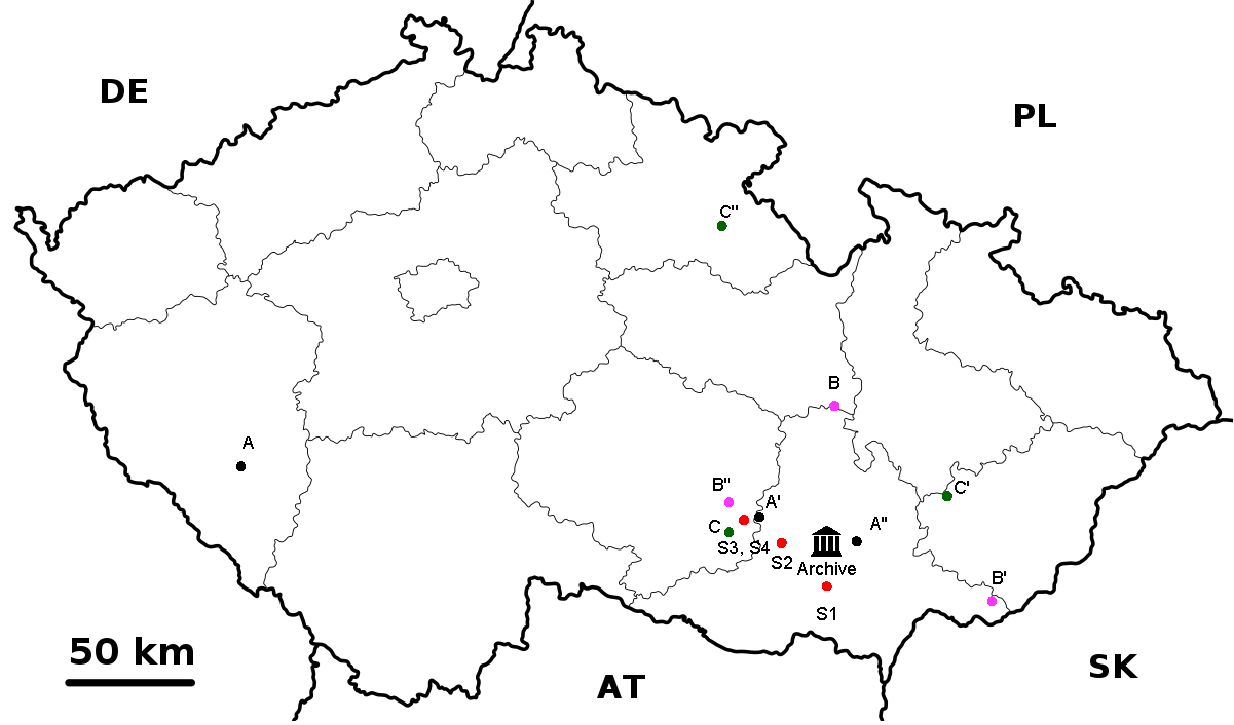
\includegraphics[scale=.6]{obrazky-figures/implementation/location_algorithm_explanation.pdf}
        \caption{Vizualizace clusterizačního algoritmu\protect\footnotemark}
\end{figure}

\footnotetext{Podkladová mapa dostupná z: \href{https://upload.wikimedia.org/wikipedia/commons/thumb/4/48/Czechia_-_outline_map.svg/1200px-Czechia_-_outline_map.svg.png}{https://upload.wikimedia.org/wikipedia/commons/thumb/4/48/Czechia\_-\_outline\_map.svg/1200px-Czechia\_-\_outline\_map.svg.png}}

\noindent
Je patrné, že se tedy jedná o~algoritmus z~třídy \texttt{fixed-point} a~tělo algoritmu tvoří primární smyčka, která čeká, dokud se neustálí střed. Jakmile dvě po sobě jdoucí iterace vrátí stejný výsledek, tak je zaručeno, že algoritmus může skončit. Jelikož vstupní parametry jsou fixní a jediný volatilní parametr je střed, tak jakmile se nezmění střed, tak neexistuje způsob, jak by algoritmus mohl vrátit jinou hodnotu, a to i v případě, kdy by algoritmus iteroval do nekonečna. V hlavní smyčce je tedy z každé kategorie vybírán nejbližší bod. K~výsledné množině se přidá aktuální střed, jenž je inicializován na bod archivu a přepočítá se nový střed. Na konci algoritmus vybere nejbližší bod z každé kategorie pro ustálený střed a danou množinu vrátí.
\begin{algorithm}
\caption{Hledání shluku lokalit}
\begin{algorithmic}[1]
    \Function{najdiShlukLokalit}{$S, C$}
        \State \textbf{Vstup}: Množina množin potenciálních oblastí $S$, počáteční střed shluku $C$
        \State \textbf{Výstup}: Množina výsledných oblastí V
        %\Repeat
        \Repeat
        %\While{Střed shluku $C$ se neustálí}
    
            \State{$ P \gets \{ p \in \mathbb{R} \times \mathbb{R}$ | $ \exists s \in S :|s| > 0 \land p = nejblizsiBod(C,s)\} \cup \{C\}$}
            
            \State{$C' \gets C$}
            \State{$C \gets spoctiStred(P)$}
        %\EndWhile
        \Until{$C \neq C'$}
        
        \State{$ V \gets \{ v \in \mathbb{R} \times \mathbb{R}$ | $ \exists s \in S: |s| > 0 \land v = nejblizsiBod(C,s)\}$}
        
        \State{\Return $V$}
    \EndFunction
\end{algorithmic}
\end{algorithm}
\newpara
V rámci shlukovacího algoritmu je využita metoda pro nalezení nejbližšího bodu z množiny k~aktuálnímu středu. Tento algoritmus spočítá vzdálenost od středu pro každý bod. Funkce vrací nejmenší prvek ze spočtené množiny $D$.

\begin{algorithm}
\caption{Hledání nejbližšího bodu}
\begin{algorithmic}[1]
\Function{nejblizsiBod}{$C,P$}    
    \State \textbf{Vstup}: Středový bod $C$, množina bodů $P$
    \State \textbf{Výstup}: Nejbližší bod $V$ k bodu $C$
    
    \State{$D \gets \{d \in \mathbb{R} \times \mathbb{R}$ | $\exists p \in P: d = spoctiVzdalenost(p, C)$ \}}
    \State{$\text{V} \gets \text{arg min}_{d \in D} d$}
    \State{\Return $V$}
\EndFunction
\end{algorithmic}
\end{algorithm}

\newpage
\noindent
Střed se spočítá jako aritmetický průměr zeměpisné šířky a výšky.

\begin{algorithm}
\caption{Výpočet středu bodů}
\begin{algorithmic}[1]
\Function{spoctiStred}{$P$}
    \State \textbf{Vstup}: Množina bodů $P$
    \State \textbf{Výstup}: Středový bod $C$
    
    \State $n \gets |P|$
    \State $ \text{sumLat} \gets \sum\limits_{p \in P} \text{p.latitude}$
    \State $ \text{sumLon} \gets \sum\limits_{p \in P} \text{p.longitude}$
    \State $C \gets \left( \frac{\text{sumLat}}{n}, \frac{\text{sumLon}}{n} \right)$
    \State \Return $C$
\EndFunction
\end{algorithmic}
\end{algorithm}
\noindent
Pro výpočet nejbližšího bodu ke středu je potřeba spočítat vzdálenost dvou bodů. Standardně se vzdálenost dvou bodů počítá pomocí Eukleidovské vzdálenosti. V~tomto případě se jedná o~souřadnice na planetě Zemi, takže je potřeba vzít v potaz, že planeta Země není rovina. V případě použití Eukleidovské vzdálenosti na zeměpisné souřadnice by výsledky nebyly korektní. Pro výpočet bude použit vzorec ze sférické trigonometrie, který se využívá například i~v~oblasti navigace. Vzdálenost dvou bodů na kouli se vypočítá pomocí Harvesinova vzorce \cite{harvesinFormula}, jenž počítá se zakřivením povrchu.


\begin{algorithm}
\caption{Výpočet vzdálenosti mezi dvěma body na Zemi pomocí Harvesinova vzorce}
\begin{algorithmic}[1]

\Function{spoctiVzdalenost}{$U,V$}
    \State \textbf{Vstup}: Bod $U$ s zeměpisnou šířkou $U_{lat}$ a délkou $U_{lon}$
    \State \textbf{Vstup}: Bod $V$ s zeměpisnou šířkou $V_{lat}$ a délkou $V_{lon}$
    \State \textbf{Výstup}: Vzdálenost $d$ mezi dvěma body
    \State{$R \gets 6371$} \Comment{Přibližný poloměr Země v kilometrech}
    \State{$\Delta\text{lat} \gets V_{lat} - U_{lat}$}
    \State{$\Delta\text{lon} \gets V_{lon} - U_{lon}$}
    \State{$\text{a} \gets \sin^2\left(\frac{\Delta\text{lat}}{2}\right) + \cos(U_{lat}) \cdot \cos(V_{lat}) \cdot \sin^2\left(\frac{\Delta\text{lon}}{2}\right)$}
    \State{$d \gets 2 \times R \times \arcsin\left(\sqrt{\text{a}}\right)$}
    \State{\Return{$d$}}
\EndFunction
\end{algorithmic}
\end{algorithm}


\section{Implementace serverové části aplikace}
 Hlavní úlohou serverové části je zpracování dat, komunikace s~databází a~poskytování dat pomocí aplikačního rozhraní. V~tomto případě je aplikace napsána v rámci aplikačního rámce Spring boot a stará se o komunikaci s relační i nerelační databází, komunikaci s~e\mbox{-mailovým} klientem a poskytování dat pomocí REST rozhraní. Jak bylo zmíněno v~návrhu, tak aplikace je monolitická a rozdělena na tři základní vrstvy.

\subsection{Ukládání dat}
Data nesplňují parametry velkých dat, a~dokonce mají i~pevnou strukturu, takže se jeví jako nejlepší nápad uložit data do standardní relační databáze. Relační databáze poskytuje konzistenci a~eliminuje redundanci dat. Problém nastává v~oblasti čtení z~databáze, kdy složitější dotazy vedou na join tabulek na základě cizích klíčů, což je náročná operace na zdroje. Výkon relační databáze se dá velmi dobře podpořit tvorbou vhodných indexovacích stromů, nicméně plně textové vyhledávání není operace, pro niž byly tyto databázové systémy vytvořeny. Tento úkol je jako stvořený pro nerelační databázi ElasticSearch, která je vhodná pro analýzu velkých dat a~vyhledávání v textu, ovšem použití NoSQL databáze by nezaručovalo konzistenci dat a~záznamy by obsahovaly mnoho redundantních informací. Existuje návrhový vzor CQRS, jenž si s~tímto dokáže poradit a~počítá v~jedné aplikaci s~použitím obou databází a~následnou synchronizací. Aplikaci využije tento návrhový vzor a~poskytne uživateli maximální komfort v~oblasti vyhledávání a~zároveň si udrží konzistentní data v~relační databázi.


\paragraph{Command Query Responsibility Segregation}\mbox{}\\
Command Query Responsibility Segregation \cite{cqrsMicrosoft, cqrsAws} je architektonický vzor oddělující operace na příkazy (commands) a dotazy (queries). 
\newpara
Příkazy jsou operace, jež modifikují stav systému, tedy přidávají či upravují data. Tato data se zpracují a uloží do relační databáze. Následně se pošle zpráva, že byla provedena změna s konkrétními daty a na straně nerelační databáze se provede synchronizace. Je potřeba mít na paměti, že použití takto oddělených databází již nesplňuje podmínky \texttt{ACID}, ale \texttt{BASE}. Toto v praxi znamená, že může nastat okamžik, kdy data mezi databázemi nejsou konzistentní, ale v budoucnu se vždy sesynchronizují. 
\newpara
Dotazy zpracovávají požadavky, které nemodifikují stav systému a pouze čtou z databáze. Tyto operace jsou prováděny nad nerelační databází, jež je v našem případě lépe optimalizovaná na plně textové vyhledávání a redukuje nutnost použití operací spojování tabulek, a to díky vhodně nastavené denormalizaci.
\newpara
Toto řešení dokáže výrazně navýšit propustnost systému a v případě, kdy jsou nasazeny dvě samostatné aplikace, jedna pro zápis a druhá pro čtení, tak se aplikace bude do budoucna i lépe horizontálně škálovat. 

\newpage
\subsection{Databázové indexy}
Jak již bylo zmíněno dříve, tak správné nastavení indexů je klíčové pro rychlé vyhledávání v rámci relační databáze. Dále budou rozepsány indexy pro jednotlivé entity, které byly odvozeny z operací v rámci repozitářů. Java Persistence API ve výchozím nastavení využívá B-strom jako typ indexu.
\newpara
Pro archivní záznam vznikl pouze jeden databázový index nad sloupcem link, jenž se využívá při upsertování záznamů ze scraperů a to ve chvíli, kdy se ověřuje, zda již daný záznam v databázi neexistuje. 
\begin{table}[H]
\begin{center}
\begin{tabular}{|l|l|l|l|}
\hline
\textbf{Název indexu} & \textbf{Indexované sloupce} &  \textbf{Unikátní} \\ \hline

idx\_link             & link                        & \cmark             \\ \hline

\end{tabular}
\caption{Indexy pro archivní záznam}
\end{center}
\end{table}

\noindent
Tabulka pro archivy obsahuje indexy nad položkami názvu a zkratky, podle nichž se archiv vždy hledá. Toto umožňuje ze scraperů posílat pouze název archivu a nemusí se tak znát přesný identifikátor daného archivu.

\begin{table}[H]
\begin{center}
\begin{tabular}{|l|l|l|l|}
\hline
\textbf{Název indexu} & \textbf{Indexované sloupce} & \textbf{Unikátní} \\ \hline

idx\_abbreviation        & abbreviation                   & \cmark             \\ \hline

idx\_name        & name                   & \cmark             \\ \hline

\end{tabular}
\caption{Indexy pro archivy}
\end{center}
\end{table}

\noindent
Záložky obsahují dva databázové indexy. Index \texttt{idx\_scan\_url} slouží pro upsert, kdy se kontroluje, zda daná záložka již neexistuje. Index \texttt{idx\_archival\_record\_id} akceleruje získávání všech záložek pro danou archiválii. 

\begin{table}[H]
\begin{center}
\begin{tabular}{|l|l|l|l|}
\hline
\textbf{Název indexu} & \textbf{Indexované sloupce} & \textbf{Unikátní} \\ \hline

idx\_scan\_url        & scan\_url                   & \cmark             \\ \hline

idx\_archival\_record\_id       & archival\_record\_id   & \xmark             \\ \hline
\end{tabular}
\caption{Indexy pro záložky}
\end{center}
\end{table}

\noindent
Jazyky obsahují pouze jeden index, a to podle názvu daného jazyka. Název by mohl být použit i jako primární klíč, bohužel při použití složených databázových indexů existuje horní limit délky a použití primárního klíče jako textového řetězce značně omezuje možnosti použití v těchto indexech.

\begin{table}[H]
\begin{center}
\begin{tabular}{|l|l|l|l|}
\hline
\textbf{Název indexu} & \textbf{Indexované sloupce} & \textbf{Unikátní} \\ \hline

idx\_name        & name                   & \cmark             \\ \hline

\end{tabular}
\caption{Indexy pro jazyky}
\end{center}
\end{table}

U lokalit existuje složený index pro kontrolu, zda se daná lokalita již v databázi nenachází. Indexy pro jednotlivé části adresy jsou určeny pro efektivní hledání adres, které dále slouží pro naplnění dropdown boxů na straně uživatelské aplikace.

\begin{table}[H]
\begin{center}
\begin{tabular}{|l|l|l|l|}
\hline
\textbf{Název indexu} & \textbf{Indexované sloupce} & \textbf{Unikátní} \\ \hline

idx\_location        & country, region, district, municipality, borough                  & \xmark             \\ \hline
idx\_region        & region                  & \xmark             \\ \hline
idx\_country        & country                  & \xmark             \\ \hline
idx\_district        & district                  & \xmark             \\ \hline

\end{tabular}
\caption{Indexy pro lokality}
\end{center}
\end{table}

Tabulka určená pro ukládání obsahuje tři databázové indexy. Index \texttt{idx\_search} slouží pro efektivní vyhledávání poznámek pro danou archiválii, a to na základě aktuálně přihlášeného uživatele. Index \texttt{idx\_search\_2} je určen pro upsert, kde se kontroluje, zda daná poznámka již neexistuje. 

\begin{table}[H]
\begin{center}
\begin{tabular}{|l|l|l|l|}
\hline
\textbf{Název indexu} & \textbf{Indexované sloupce}  & \textbf{Unikátní} \\ \hline

idx\_archival\_record\_id        & archival\_record\_id                   & \xmark             \\ \hline

idx\_search        & archival\_record\_id, accessibility, user\_id                   & \xmark             \\ \hline

idx\_search\_2        & scan\_url, user\_id, accessibility                   & \cmark             \\ \hline

\end{tabular}
\caption{Indexy pro poznámky}
\end{center}
\end{table}

Indexy pro uživatele jsou nastaveny tak, aby aplikace mohla efektivně vyhledávat uživatele při ověření JWT tokenu. Dále jsou vytvořeny indexy pro jednotlivé hashe, v případě že si chce uživatel ověřit účet, tak se na základě tohoto hashe dohledává účet.

\begin{table}[H]
\begin{center}
\begin{tabular}{|l|l|l|l|}
\hline
\textbf{Název indexu} & \textbf{Indexované sloupce} & \textbf{Unikátní} \\ \hline

idx\_email        & email                   & \cmark             \\ \hline

idx\_is\_verified\_and\_email        & email, isVerified     & \cmark             \\ \hline

idx\_verify\_hash        & verify\_hash                   & \cmark             \\ \hline

idx\_password\_reset\_hash        & password\_reset\_hash                   & \cmark             \\ \hline

\end{tabular}
\caption{Indexy pro uživatele}
\end{center}
\end{table}
 
\paragraph{Synchronizace databází}\mbox{}\\
Relační i nerelační databáze je nastavená, nyní je třeba zařídit jejich vzájemnou synchronizaci. Při implementaci čistého CQRS návrhové vzoru se uvažují dvě separátní služby, které spolu komunikují zasíláním zpráv. Tento typ implementace by za cenu lepší škálovatelnosti přinášel značnou režii navíc. Vzhledem k tomu, že se pro mapování objektů mezi relační databází a objekty v Javě využívá aplikační rámec Hibernate, tak je použita nadstavba Hibernate-search \cite{hibernateSearch}. Hibernate musí sledovat změny na objektech a v případě ukončení transakce propíše změny do databáze. To, že sleduje změny, je v tomto případě klíčové, jelikož to je přesně to, co je potřeba pro synchronizaci daných databází. Hibernate-search po správné konfiguraci propisuje změny do indexů v Elasticseach databázi. Všechna data jsou uložena v relační databázi, sloužící jako zdroj faktů, a v rámci Elasticsearch se udržují pouze indexační stromy bez samotných dat. Dotazy tedy najdou identifikátory v nerelační databázi a následně je Hibernate vyhledá v~relační databázi. Tento přístup je sice pomalejší než duplikování dat do nerelační databáze, ale má nižší paměťové nároky. V~případě, že by se data duplikovala do nerelační databáze, tak by musely být nastaveny atributy pro projekci.

\subsection{Bezpečnost}
V návrhu se vyskytuje pojem přihlášený uživatel, a proto je na místě řešit bezpečnost a~jak bude probíhat autentizace uživatelů. Při použití architektury klient-server se může použít HTTP Basic autentizace. Problém tohoto přístupu je, že se heslo posílá v~čitelné podobě, a~jelikož protokol HTTP je bezstavový, tak se musí posílat při každém požadavku na server. Tento problém může být částečně vyřešen použitím šifrovaného spojení pomocí HTTPS, ovšem stále je nutné řešit problém uchování hesla na straně klienta, jelikož ho klient musí přiložit ke každému požadavku. Z hlediska bezpečnosti se jeví daleko praktičtější použití token-based autentizace. Token-based autentizace vyžaduje poslání citlivých údajů pouze jednou a po provedení autentizace se vygeneruje token, jenž bude uživatel používat dál pro autorizaci. Dalším přístupem je použití OAuth, který pro autentizaci používá služby třetích stran. Tato služba je použita v mnoha systémech, kdy se uživatelé přihlašují pomocí Facebook nebo Google účtu bez registrace v~rámci dané aplikace. Pro požadavky této aplikace se jeví jako nejlepší řešení použít \texttt{token-based} autentizaci, konkrétně JSON Web Token \cite{jwt}, který je definován standardem RFC 7519. Token se skládá z~hlavičky, těla a~podpisu. Hlavička obsahuje informace o typu tokenu a~použitém algoritmu, jímž byl token podepsán. Tělo obsahuje uživatelská data ve formátu JSON. Třetí část je podpis dat tokenu a~slouží k~ověření autenticity a~integrity tokenu.

\begin{figure}[htbp]
    \centering
        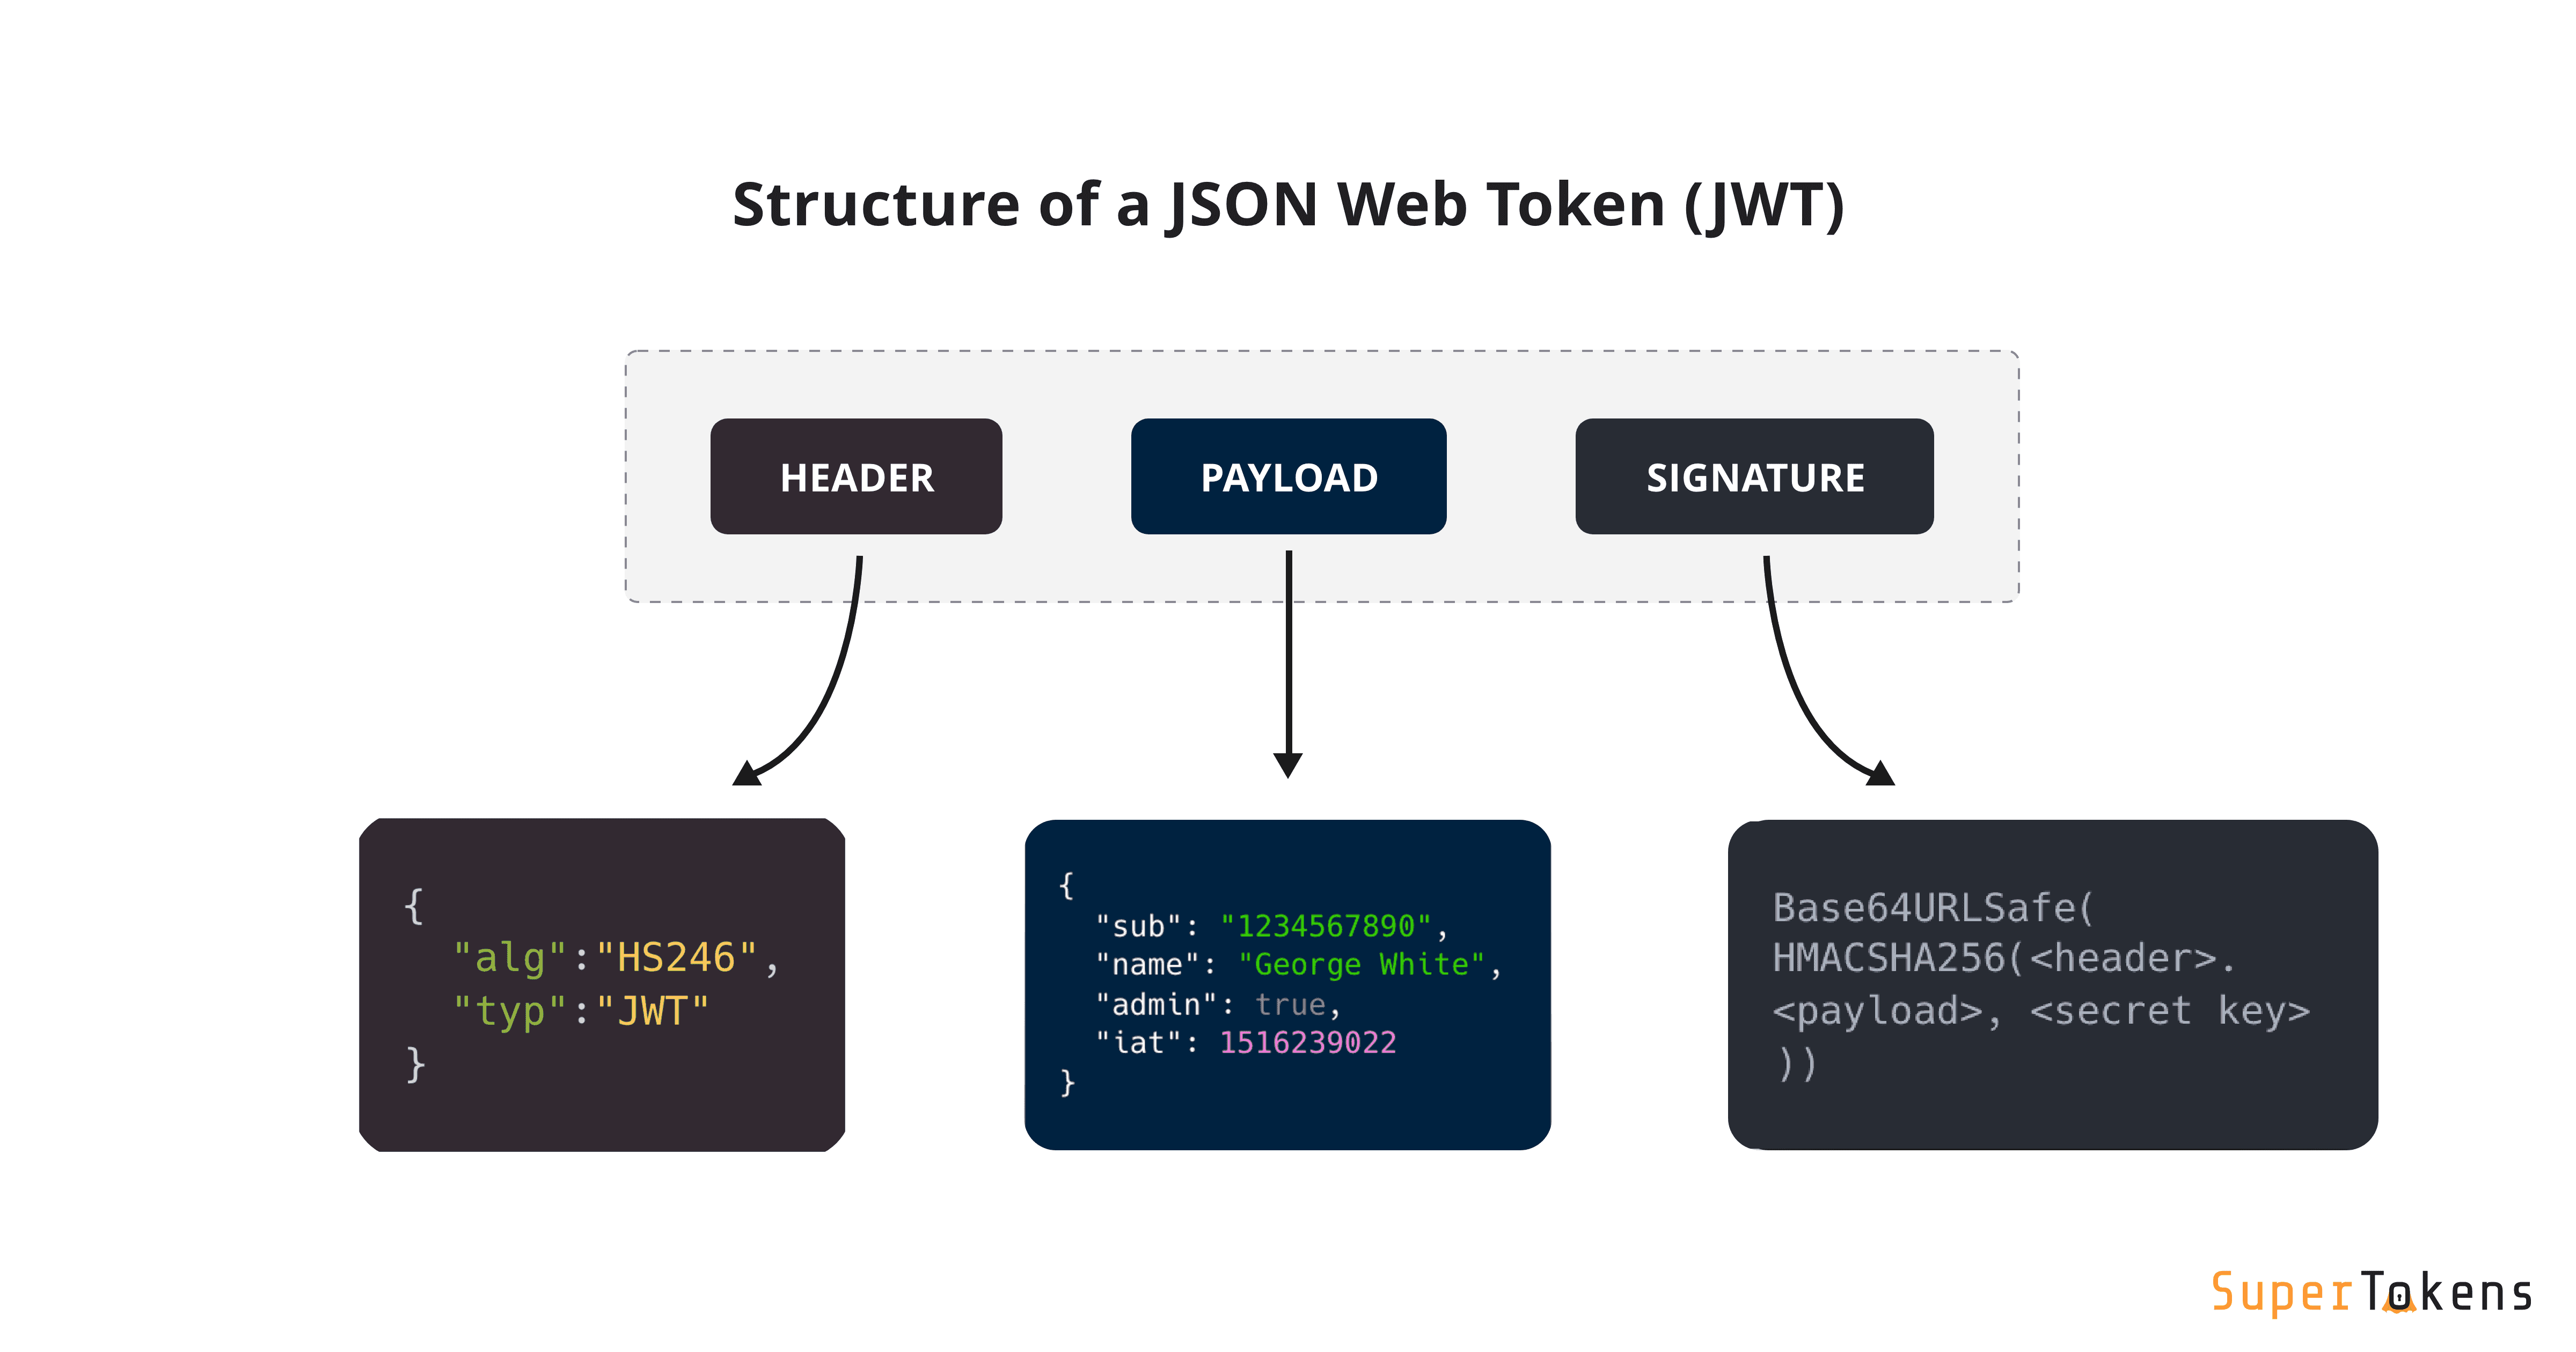
\includegraphics[scale=.09]{obrazky-figures/implementation/jwt-structure.png}
        \caption{Struktura JWT tokenu\protect\footnotemark}
\end{figure}

\footnotetext{Diagram dostupný z: \href{https://supertokens.com/static/b0172cabbcd583dd4ed222bdb83fc51a/9af93/jwt-structure.png}{https://supertokens.com/static/b0172cabbcd583dd4ed222bdb83fc51a/9af93/jwt-structure.png}}

\noindent
Na obrázku \ref{fig:jwt-communication} lze vidět ukázku použití tokenu v komunikaci mezi klientem a serverem. Uživatel provede přihlášení, server ověří údaje a vygeneruje token. Tento token si klient uchová a použije při dalších požadavcích vyžadujících autorizaci. Klient si sice musí informaci pamatovat stejně jako u HTTP basic, ale v případě, že se útočník dostane k tokenu, tak ten zpravidla platí po omezenou dobu a bez znalosti hesla není útočník schopný vygenerovat nový token, a tím prodloužit platnost.

\begin{figure}[htbp]
    \centering
        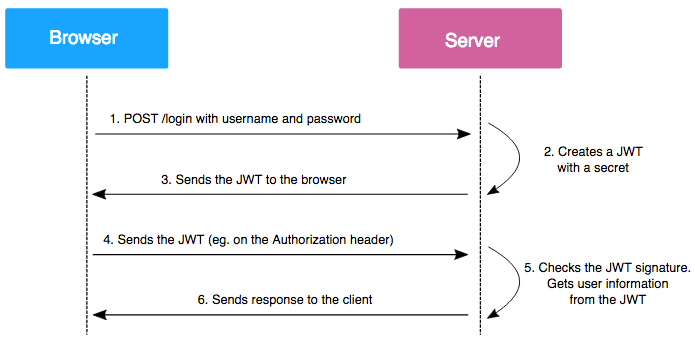
\includegraphics[scale=.6]{obrazky-figures/implementation/jwt_communication.png}
        \caption{Ukázka použití JWT tokenu\protect\footnotemark}
        \label{fig:jwt-communication}
\end{figure}

\footnotetext{\href{https://www.vaadata.com/blog/wp-content/uploads/2016/12/JWT_tokens_EN.png}{https://www.vaadata.com/blog/wp-content/uploads/2016/12/JWT\_tokens\_EN.png}}

\subsection{Odesílání e-mailů}
Požadavky jako ověřování uživatelů a resetování hesla vyžadují implementovat podporu pro komunikaci se SMTP serverem. V rámci produkční verze je využit SMTP server od Gmailu, ovšem v době implementace není vhodné zasílat e-maily na skutečné adresy z důvodu ladění a možného nechtěného spamu. Za tímto účelem byl použit nástroj Mailhog, který se tváří jako SMTP server, ovšem místo skutečného odesílání e-mailů je pouze zachytává a zobrazuje skrze webové rozhraní. Pro samotnou komunikaci se serverem bylo využito JavaMail API. Veškeré nastavení e-mailového serveru je skrze proměnné prostředí a konfiguraci je tedy možné provést bez zásahu do zdrojového kódu.


\section{Dokumentace}
V době, kdy programátor tvoří nějaký program nebo algoritmus, tak mu je úplně jasné, jak daný kus kódu funguje. Problém nastává v případě, že má do projektu začít přispívat nový kolega nebo se k projektu vývojář vrací po delší době. Kvůli těmto aspektům je dokumentace velmi důležitou součástí zdrojových kódů. Pro Javu existuje dokumentační nástroj Javadoc, který na úkor striktního formátu dokumentačních komentářů vygeneruje celou programovou dokumentaci ve formě webové stránky. Dokumentaci je možné vygenerovat pomocí Maven pluginu Javadoc.


\section{Implementace klientské aplikace}
Klientská aplikace je napsána v reaktivním JavaScriptovém  aplikačním rámci React.JS \cite{reactDev}, který se primárně stará o~vizualizaci dat a~poskytuje grafické uživatelské rozhraní pro naše aplikační rozhraní. React.JS využívá deklarativní a~komponentově orientovaný přístup, což znamená, že celý pohled systému se dekomponuje na jednotlivé znovupoužitelné komponenty. V~rámci komponent se deklaruje jejich chování a~rozložení na základě stavu. Každá komponenta může používat další komponenty, což umožňuje hierarchicky budovat nové rozhraní. Komponenta má dále stav a~vlastnosti, jež si udržuje v průběhu celého svého životního cyklu. Životní cyklus komponenty zahrnuje více fází, mezi něž patří inicializace, aktualizace a odstranění. Na tyto fáze životního cyklu je možné navázat obslužné metody, které například při inicializaci mohou provést stažení požadovaných dat a~naopak u odstranění po sobě uklidit. Ke komponentě může náležet soubor s definicí stylů. V~případě, že má komponenta obsahovat logiku, tak je tato logika vytknuta do separátního hooku, díky čemuž je dodržen princip jedné zodpovědnosti. React pracuje nad virtuálním DOM stromem, při každé změně stavu aplikace se vygeneruje nový virtuální DOM strom, který se porovná s~aktuálním, a~nahradí se pouze změněné části. Toto řešení má pozitivní dopad na výkon aplikace.
\newpara
JavaScript je dynamicky typovaný, což znamená, že proměnné mohou měnit svůj typ za běhu programu. Pro větší aplikace je lepší použít typový systém umožňující psát robustnější kód a snižovat pravděpodobnost chyb. TypeScript je opensource nadstavba od Microsoftu pro jazyk JavaScript. Tato nadstavba přidává statické typování. Největší nevýhoda použití TypeScriptu spočívá v~použití knihoven, které nemají vytvořené definice typů pro TypeScript. V~tomto případě existují tři možnosti: najít alternativní knihovnu s podporou TypeScriptu, vytvořit definici typů nebo komponentu, v níž má být knihovna použita přepsat do JavaScriptu. První volba je nejrozumnější, pokud daná alternativa existuje. Problém u poslední alternativy nastává v případě použití ESLint, který v konfiguraci může zakazovat použití JavaScriptových komponent, a proto je potřeba tuto konfiguraci upravit.
\newpara
Pro kontrolu kvality kódu byl zvolen nástroj ESLint, který provádí statickou analýzu TypeScriptového kódu. Nástroj se soustředí na nalezení a~odstranění chyb, konvenční nedostatky a~eliminaci anti návrhových vzorů. ESLint funguje na základě předdefinovaných pravidel, a~v~tomto projektu byla zvolena konfigurace, která se využívá ve společnosti Google.
\newpara
Uživatelské rozhraní by mělo být konzistentní napříč celým systémem a~mělo by používat jednotný vzhled u jednotlivých komponent. Cílem tvorby nových systémů není znovu objevovat kolo. Existují různé sady předdefinovaných komponent, které se dají použít při tvorbě nových pohledů v systému. Pro tento projekt byla zvolena knihovna \href{https://primereact.org/}{PrimeReact} nabízející dostatečnou paletu komponent. Vzhled výsledné aplikace vychází z~návrhu v~nástroji Figma a ukázky uživatelského rozhraní jsou v~rámci přílohy \ref{appendix:client-ui} Ukázka grafického uživatelského rozhraní výsledné aplikace.
\newpara
Pro komunikaci s~API pomocí protokolu HTTP se používá knihovna Axios. Samotné volání Axios je zapouzdřeno a~komponenta k~němu přistupuje skrze Redux hooky. Jak bylo zmíněno v popisu aplikačního rámce React.JS, tak každá komponenta má interní stav, na základě kterého se provádí překreslení. Problém nastává, když více komponent má sdílet stejný stav. Toho se dá docílit předáváním hodnot skrze parametry komponent, což vyžaduje, aby definice tohoto stavu byla v~komponentě, jež je kořenem podstromu DOM, v~němž jsou všechny komponenty s~touto závislostí. Definování proměnné v~komponentě, která danou závislost nevyžaduje, je nepřehledné a nepřenositelné. Lepší alternativou je použíti React konstruktu \texttt{kontext}, kde se definuje rozsah platnosti daného \texttt{kontextu} a~následně si komponenty skrze něj mohou sdílet data. Robustním řešením, které kombinuje možnost sdílet data napříč komponentami a~zároveň zapouzdřuje komunikaci s~API, je Redux. Redux definuje centrální úložiště dat \texttt{store} a~striktně odděluje operace pro čtení a~zápis. V~případě, že má dojít k~úpravě dat ve \texttt{storu}, tak se volá přes \texttt{dispatch hook} konkrétní akce. Akce může obsahovat volání API a~následně vytvoří zprávu pro \texttt{reducer}. Zpráva pro \texttt{reducer} obsahuje data a~typ. Typ akce musí být unikátní pro celou aplikaci. Následně Redux prochází jednotlivé \texttt{reducery}, jež jsou implementovány formou switch konstrukce. Jakmile je konkrétní obslužná funkce nalezena, tak se provede změna stavu v~\texttt{store}. V~případě, že komponenta chce číst hodnotu ze \texttt{store}, tak použije \texttt{selector hook}, který začne odebírat data z~centrálního úložiště, a~v~případě změny závislých dat ve \texttt{storu} je daná komponenta překreslena. Tato základní architektura je rozšířena o~\texttt{selectorHook} a~\texttt{actionHook}, které zapouzdřují jednotlivé akce a~selectory a~eliminují nutnost použití Redux hooků přímo v~komponentech. Pomocí této abstrakce lze přímo volat v~komponentech metody a~tím dochází k~plnému odstínění od architektury Reduxu.

\begin{figure}[htbp]
    \centering
        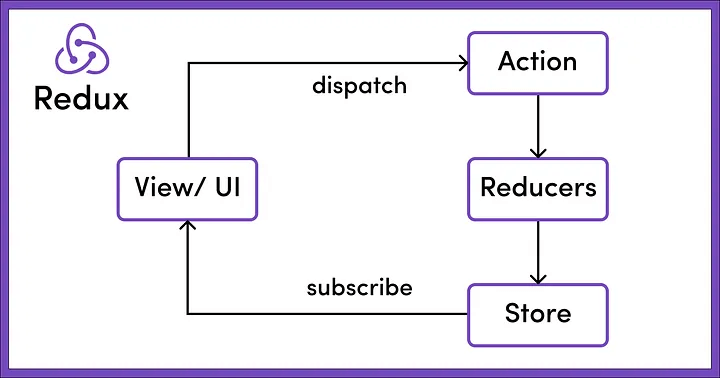
\includegraphics[scale=.6]{obrazky-figures/implementation/redux_architecture.png}
        \caption{Architektura Redux\protect\footnotemark}
\end{figure}

\footnotetext{ \href{https://miro.medium.com/v2/resize:fit:720/format:webp/1*EV1KQifr5KwiupJ9q7tdxA.png}{https://miro.medium.com/v2/resize:fit:720/format:webp/1*EV1KQifr5KwiupJ9q7tdxA.png}}

\noindent
Jak bylo popsáno v úvodu práce, tak archivy poskytují naskenované archiválie v různých formátech, a to včetně dlaždicových. Pro vizualizaci těchto dlaždicových snímků je využita opensource knihovna OpenSeaDragon \cite{openSeaDragon}, která má nativní podporu pro zobrazování dlaždicových formátů. Kromě samotného zobrazení obsahuje knihovna možnosti pro navigaci, přibližování a posouvání po snímku. Základní funkcionalita OpenSeaDragon lze rozšířit díky zásuvným modulům. V této práci je využit zásuvný modul mající podporu pro Fabric.JS vrstvu. Fabric.JS \cite{fabricJs} je knihovna pro práci s kreslením a manipulací s grafickými prvky v~rámci HTML5 canvasu. Bohužel použití těchto knihoven hlásilo chyby a~bylo nutné referenční knihovnu forknout\footnote{\href{https://github.com/sestakp/OpenseadragonFabricjsOverlay}{https://github.com/sestakp/OpenseadragonFabricjsOverlay}} na githubu upravit a následně publikovat\footnote{\href{https://www.npmjs.com/package/@sestakp/openseadragon-fabricjs-overlay}{https://www.npmjs.com/package/@sestakp/openseadragon-fabricjs-overlay}} na platformě npm.

\begin{figure}[htbp]
    \centering
        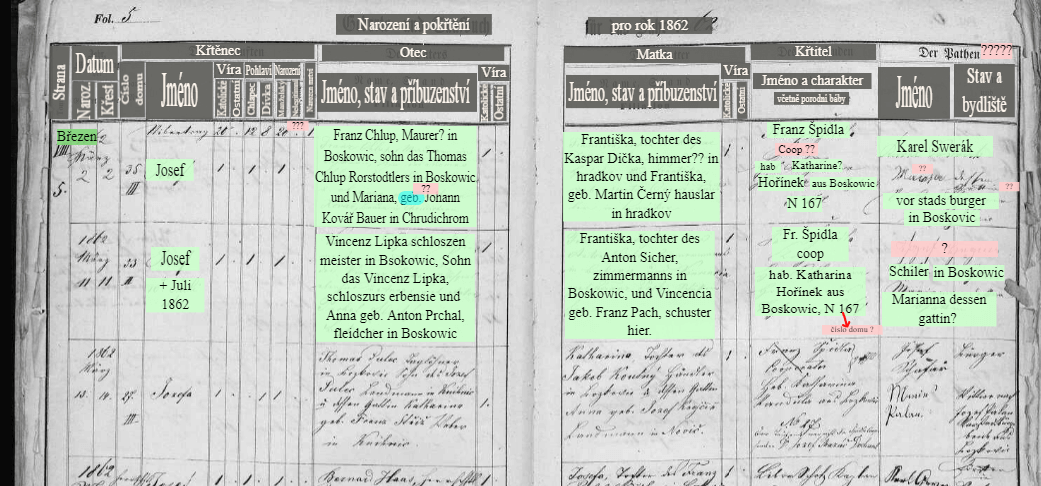
\includegraphics[scale=.4]{obrazky-figures/implementation/notesExample.PNG}
        \caption{Ukázka archiválie s anotacemi}
\end{figure}

\section{Implementace proxy pro snímky archiválií}
Pokud by byl použit externí odkaz na snímek přímo z webové aplikace a ta by se jej pokusila stáhnout, tak by požadavek skončil s HTTP stavovým kódem 403 – zamítnuto. Na vině je bezpečnostní mechanismus CORS \cite{cors}, který je implementován ve webovém prohlížeči. Bezpečnostní mechanismus CORS se spouští v případě, kdy načtená webová stránka z jedné domény (origin) požádá o zdroje z jiné domény. Klient v požadavku tedy zasílá hlavičku \texttt{origin} a server následně musí k odpovědi přidat hlavičku \texttt{Access-Control-Allow-Origin}. Prohlížeč následně porovná, že se tyto hodnoty rovnají a v opačném případě zamítne přístup k datům. 
\newpara
S touto mechanikou je potřeba počítat i při implementaci klientské aplikace, jež komunikuje se separátní serverovou aplikací. Zde je problém lehce řešitelný, jelikož na straně serveru stačí správně nastavit odesílání hlaviček, které se ke CORS vztahují. Problém nastává v případě, kdy je třeba přistoupit k cizímu API. V případě, že má cizí API omezený seznam povolených klientů, tak toto chování nelze změnit bez zásahu do kódu.
\newpara
Jednoduchým řešením je tvorba samostatné webové aplikace, která se bude chovat jako proxy. Proxy je takový prostředníček, jenž vezme požadavek, přepošle ho a následně vrátí odpověď.
Celé řešení je napsáno pomocí JavaScriptového aplikačního rámce pro tvorbu aplikačních rozhraní Express.JS.


\begin{figure}[htbp]
    \centering
        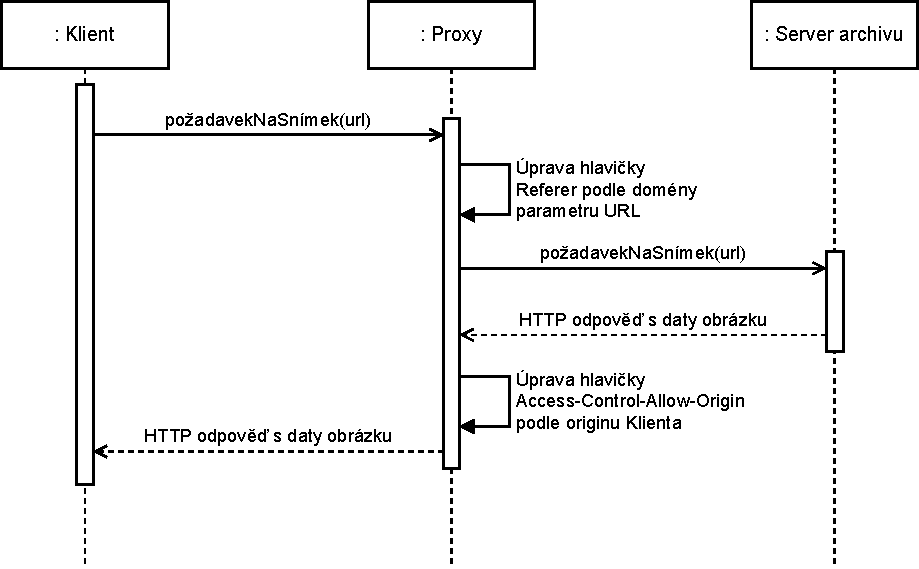
\includegraphics[scale=1]{obrazky-figures/implementation/image_proxy_communication_diagram.pdf}
        \caption{Ukázka komunikace pomocí proxy}
\end{figure}

\newpage
\section{Kontejnerizace}
Celý systém se skládá z několika separátních služeb, kde každá služba má svůj seznam závislostí, které je potřeba nainstalovat a udržovat. U každé závislosti se mohou vyskytnout problémy s nekompatibilním nastavením prostředí a verzemi jednotlivých knihoven. V neposlední řadě je zde otázka bezpečnosti, jelikož aplikace jsou spuštěny v izolovaném prostředí a pro potencionální nebezpečnou aplikaci je tedy složitější se dostat do hostujícího stroje. Kontejnerizace je lehčí varianta virtualizace, jež díky využívání hostitelského operačního systému není tak náročná na výpočetní výkon. V našem případě využijeme platformu Docker.

\subsection{Docker}
Docker \cite{dockerOverview} je open source platforma pro vývoj, doručení a provozování aplikací. Pomocí Dockeru lze každou aplikaci zabalit a spustit v separátním kontejneru. Na jednom stroji je následně možné provozovat více kontejnerů současně. Pro každou aplikaci nebo službu, která má být nasazena přes Docker, je třeba vytvořit \texttt{Dockerfile}. V rámci každého \texttt{Dockerfile} je nutné specifikovat Docker Image, což je základní balík obsahující závislosti vždy pro konkrétní aplikaci, jako je například Python nebo běhové prostředí pro Javu. Následuje sekvence příkazů, která většinou provádí nakopírování zdrojových souborů, stažení závislostí, překlad a~spuštění aplikace. Většinou se po takto nasazené službě vyžaduje interakce, proto se vytvoří tunel portu z daného kontejneru. Tuto situaci si lze představit následovně – běží-li v kontejneru webový server na portu 80, tak lze port vytunelovat na libovolný neobsazený hostitelský port a přistoupit tak k~aplikaci, která je nasazená v kontejneru. Pokud je potřeba, aby kontejner nepřišel o svoje data v případě restartu, tak lze na daný kontejner napojit volume. Jak bylo zmíněno výše, tak jednotlivé kontejnery jsou vzájemně izolované, což v případě distribuovaných systémů znemožňuje komunikaci mezi jednotlivými službami. Za tímto účelem lze v rámci Dockeru vytvořit síť obdobně jako volume. Následně tak všechny kontejnery ve stejné síti mohou mezi sebou komunikovat.

\subsection{Docker compose}
Použití jednotlivých \texttt{Dockerfile} sice odstiňuje od instalování závislostí, ale pořád osoba, jež systém instaluje, musí mít povědomí o architektuře aplikace. Je třeba vytvořit jednotlivé volumes, případně síť, a znát konkrétní porty jednotlivých kontejnerů, které je nutné vytunetoval. Pro úspěšné nasazení nezasvěcenou osobou by bylo nutné vytvořit metodiku, jež daný proces popisuje, ale stále zde hrozí, že osoba metodiku špatně interpretuje nebo udělá chybu. Pro úplné odstínění problémů s nasazením aplikace je použit konfigurační \texttt{YAML} soubor \texttt{docker-compose}, kde jsou specifikovány jednotlivé kontejnery a jejich \texttt{Dockerfily}. Dále je zde nakonfigurováno všechno přidružené nastavení, jako jsou zmíněné porty, volumes a síť. V případě, kdy je celý systém popsán v jednom \texttt{Docker compose} konfiguračním souboru, pak danou síť není třeba tvořit, jelikož pro každý \texttt{Docker compose} existuje síť implicitně. Následně stačí systém jako celek nasadit jedním příkazem \texttt{docker compose up}, který může být doplněn o přepínač \texttt{-d}, což daný příkaz spustí na pozadí, a~\texttt{--build} pro znovu přeložení aplikace v případě, že nahráváme novou verzi. 

\newpage
\subsection{Architektura Docker}
Docker používá architekturu klient-server, kde klient s daemonem komunikuje pomocí UNIX socketů, síťového rozhraní nebo REST API. Klient se může připojit na lokálního i vzdáleného daemona. Jak bylo zmíněno, tak v každém \texttt{Dockerfile} je specifikován Docker image, který se stahuje ze vzdálených Registry. Jakmile se daný Docker image stáhne, tak se uloží na disk a je dostupný pro opakované použití bez nutnosti opětovného stahovaní. Jakmile daemon provede stažení Docker image, tak se paralelně spustí \texttt{Dockerfily} jednotlivých služeb a následně se vytvoří kontejnery.

\begin{figure}[htbp]
    \centering
        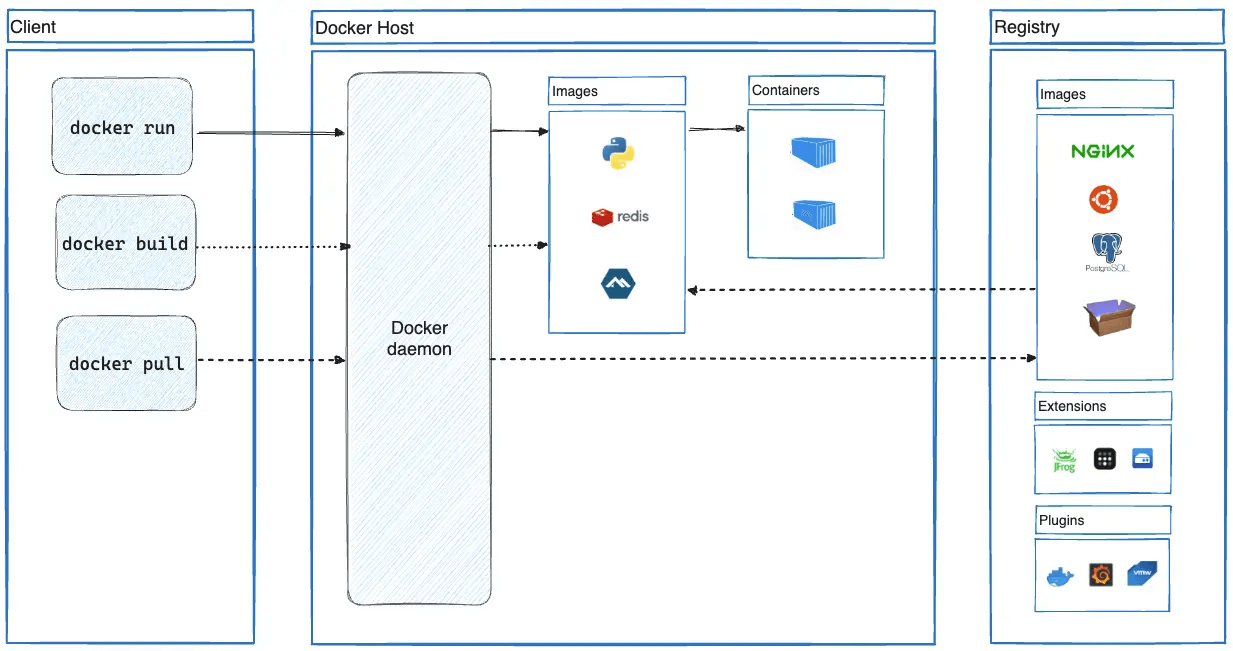
\includegraphics[scale=.3]{obrazky-figures/implementation/docker-architecture.png}
        \caption{Architektura Dockeru \footnotemark}
\end{figure}
\footnotetext{Obrázek pochází ze stejného zdroje jako informace o Dockeru.}